\section{Extended Multi-Lingual Semantic Framework}
\label{sec:framework}

Cross-language CES comparison poses the key technical difficulty in scaling up the Phase~1 approach. Since the extraction scripts of Phase~1 created language-specific semantic labels out of CPG loop node types, structurally similar loops in distinct languages were translated into disjoint pattern vectors, which made cross-language comparison meaningless. The following three specific contributions are designed to overcome the said difficulty: a Context Normalization Protocol capable of solving semantic label mismatch problem in the context of code similarity evaluation, expanded CES taxonomy incorporating C++ STL idioms and Java API patterns, and asymmetric Tversky formula compensating for verbosity discrepancy between C and Java programming languages. Figure~\ref{fig:architecture_pipeline} shows the architecture of the extended pipeline.

\begin{figure*}[!t]
    \centering
    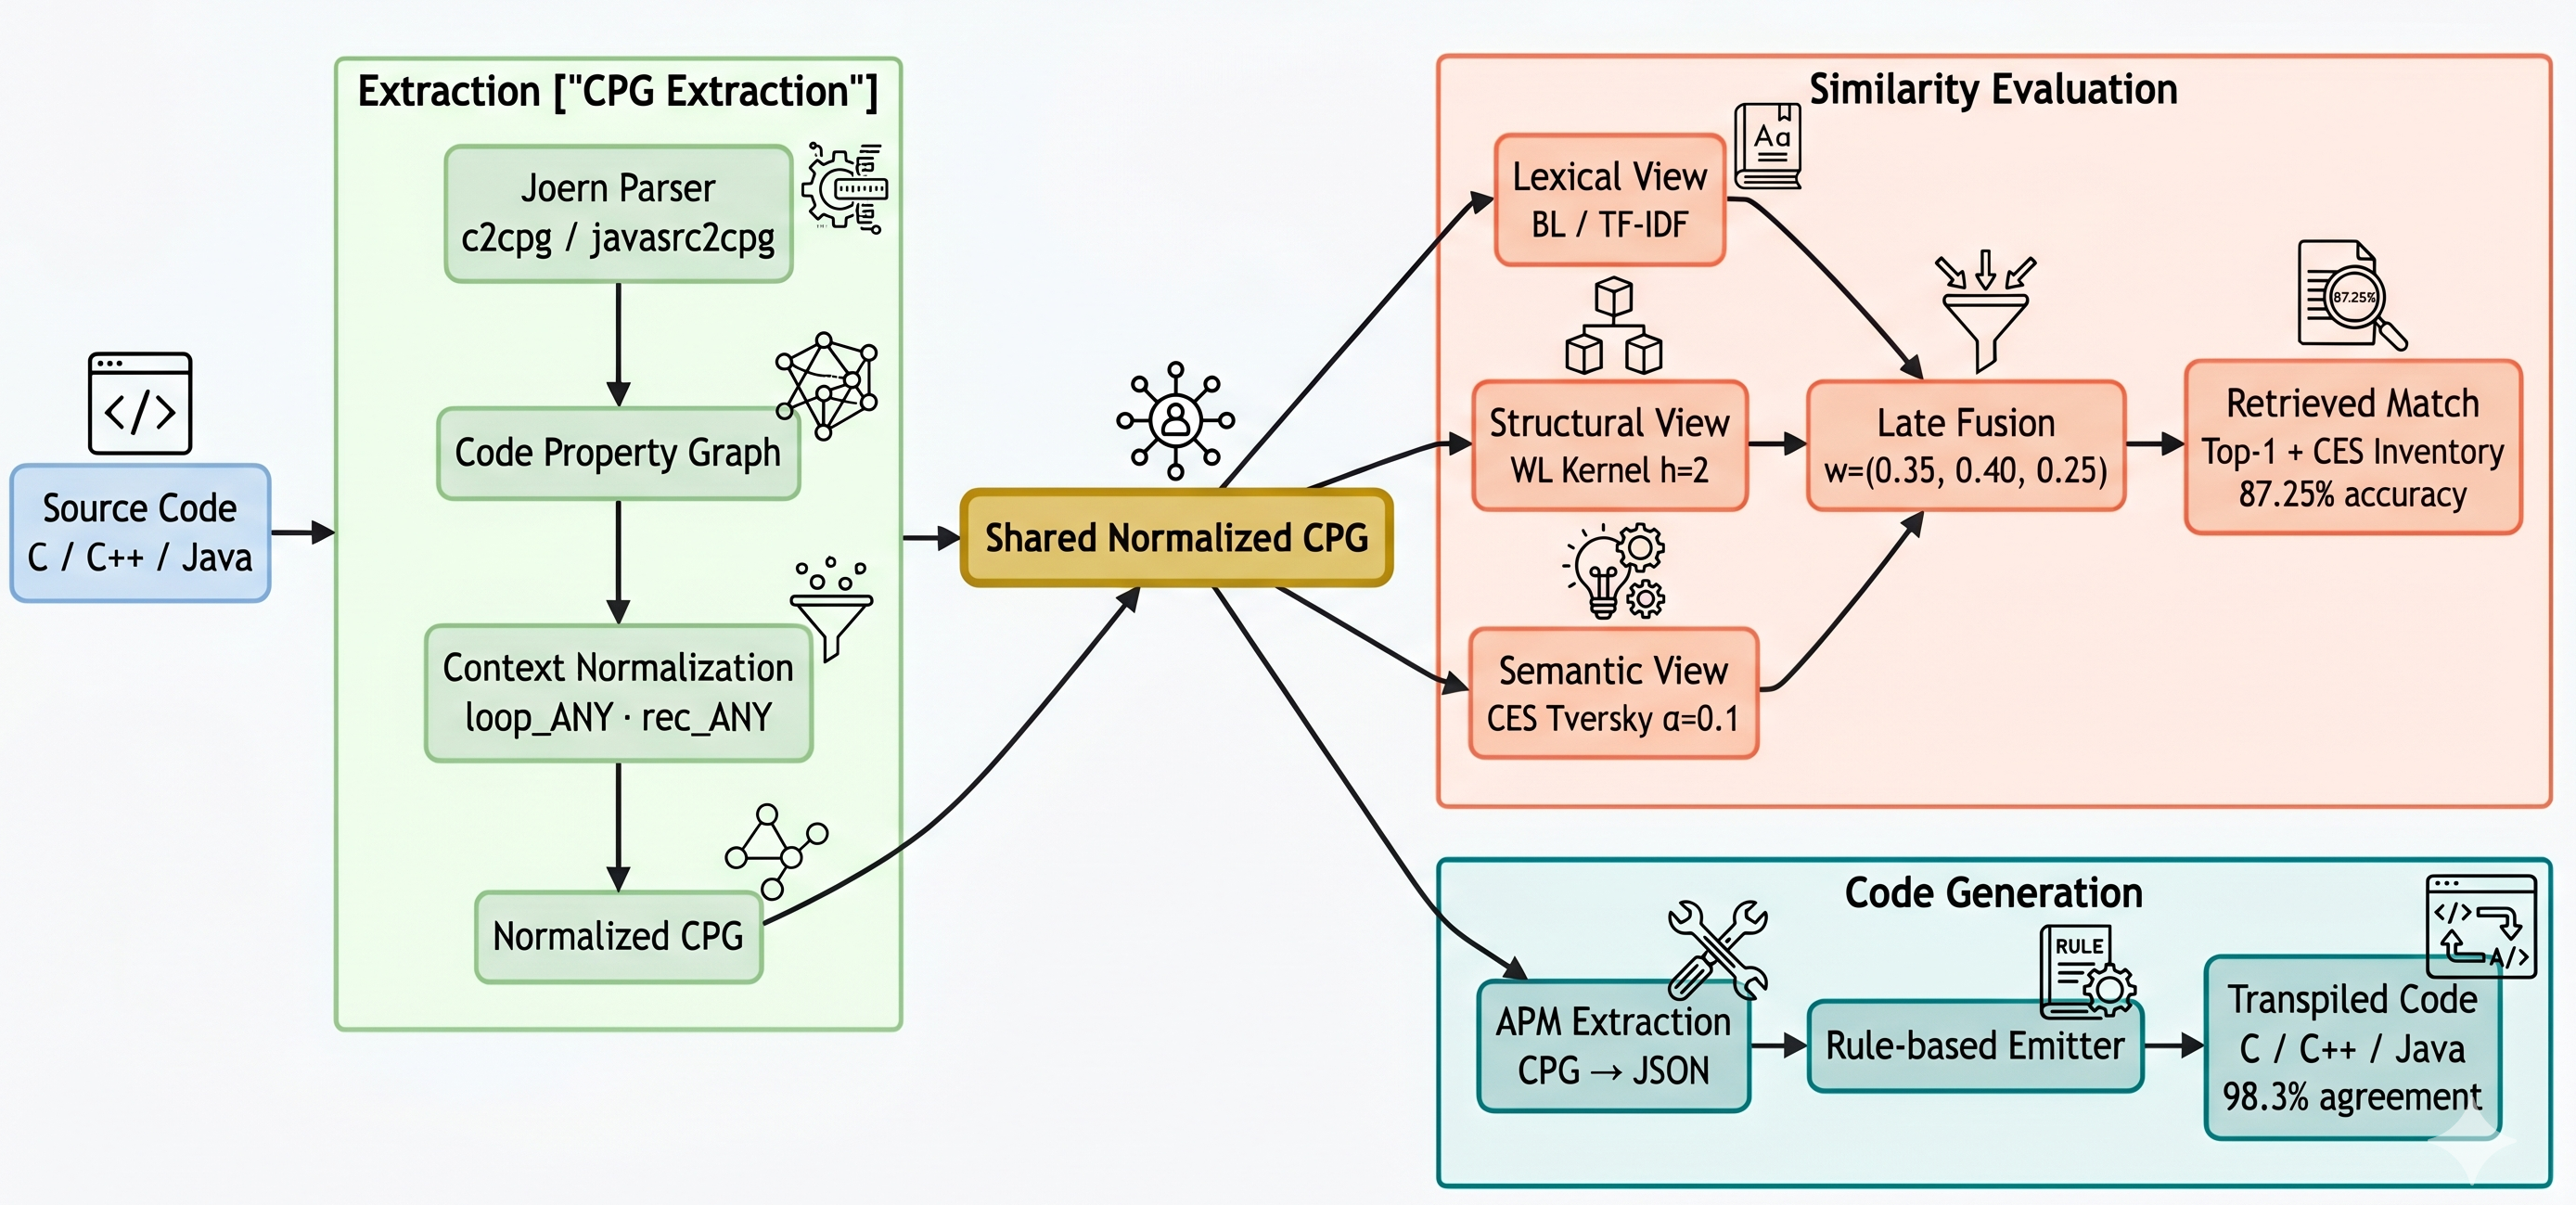
\includegraphics[width=\textwidth]{IEEE_Access_Draft/Sections/architecture1.png}
    \caption{Extended multi-lingual pipeline. Source code in C, C++, or Java is parsed into a Code Property Graph via Joern's language-specific frontends, each sharing a common CPG node schema. The Context Normalization layer maps language-specific constructs to abstract semantic tokens. The pipeline branches into Similarity Evaluation (three-view late fusion) or APM-based Code Generation (deterministic rule-based emission). The two branches share the graph representation but operate as architecturally independent extraction pathways with no shared data flow. Internal weight values shown denote the grid-search evaluation increments used to optimize the late-fusion parameters.}
    \label{fig:architecture_pipeline}
\end{figure*}

\subsection{Phase~1 Architecture and CPG Unification}
\label{subsec:phase1_base}
In Phase~1, we established a three-view CPG-based framework for measuring algorithmic similarity in single-language C educational assignments, achieving 88.5\% top-1 retrieval accuracy on 104 programs. The framework combines: (i) a \textit{Baseline view} computing TF-IDF similarity over normalized code identifiers; (ii) a \textit{Structural view} computing Weisfeiler-Lehman graph kernel similarity over CPG AST nodes; and (iii) a \textit{Semantic view} based on Computation Evolution Signatures (CES). These three views are combined using a linear weighted late fusion with the weights set to $(w_{BL}, w_{WL}, w_{CES}) = (0.35, 0.40, 0.25)$, tuned by exhaustive grid search over a dataset of 104 C-language submissions collected on the same 20 problems corpus as in Phase~2. \textcolor{blue}{For a detailed derivation of Phase~1, we refer the reader to the original manuscript;} this section focuses on the Phase~2 extensions.

The framework does not use back-propagation; TF-IDF weighting is done based on deterministic fitting using corpus statistics, and the APM rule base is hand-authored. To support multi-language input, Joern's language-specific parsers map C, C++, and Java source code into a common CPG schema: C and C++ share a single \texttt{c2cpg} frontend, while Java uses the separate \texttt{javasrc2cpg} frontend. This structural disparity, in which programs in C and C++ yield almost identical vocabularies of CPG node types, while Java programs are mapped to CPG by a separate parser, is listed in Section~\ref{subsec:threats} as a validity threat, and explains the need for the directional stratification of results discussed in Section~\ref{sec:results}.

\subsection{Context Normalization Protocol}
\label{subsec:context_norm}
The primary barrier to cross-language CES comparison is language-bound context labeling: in Phase~1, extraction scripts generated CES context labels directly from CPG loop node types, so a \texttt{for}-loop produced \texttt{loop\_FOR} and a \texttt{while}-loop produced \texttt{loop\_WHILE}. Thus two semantically equal cross-language programs would consequently yield two CES vectors containing non-equal context labels and, thus, be incomparable.

The Context Normalization Protocol solves this problem through abstraction of syntactic forms to semantics at the time of creating graphs. As a result, all forms of loops, including \texttt{for}, \texttt{while}, \texttt{do-while}, and C++ range-based \texttt{for} loops, are collapsed to \texttt{loop\_ANY}, while all recursive functions are abstracted to \texttt{rec\_ANY}. All other syntactic constructs that have no analogs in the shared taxonomy are filtered from the pattern vector during the process. The normalization is completely deterministic; no language mapping is needed, neither bilingual corpus nor any intermediate representation but the CPG itself. The resulting vectors are directly comparable across language boundaries, as illustrated in Table~\ref{tab:context_norm_illustration}.

\textbf{STL call injection:} In the case where there is no loop node in the CPG associated with the STL call (such as \texttt{std::accumulate}), the pattern mapping of the STL patterns table recognizes the corresponding \texttt{CallExpression} node and inserts a placeholder \texttt{loop\_ANY} token prior to pattern recognition. Algorithm~\ref{alg:stl_injection} presents the detailed process, including the filtering path for out-of-coverage constructs.

\begin{algorithm}[t]
\caption{STL Call Injection Protocol}
\label{alg:stl_injection}
\begin{algorithmic}[1]
    \For{each $\text{node} \in \textsc{Cpg.Nodes}()$}
        \If{$\text{node.type} = \texttt{CallExpression}$}
            \If{$\text{node.name} \in \textsc{Stl\_Map}$}
                \State $\text{pattern} \leftarrow \textsc{Stl\_Map}[\text{node.name}]$
                \State $\textsc{InjectContext}(\text{node},\ \texttt{loop\_ANY})$
                \State $\textsc{EmitCes}(\texttt{loop\_ANY},\ \text{pattern})$
            \Else
                \Comment{Unmapped idiom: filter node}
                \State $\textsc{MarkFiltered}(\text{node})$
            \EndIf
        \EndIf
    \EndFor
\end{algorithmic}
\end{algorithm}

\textbf{Protocol coverage:} The normalization covers all standard C/C++ loop constructs, all Java loop forms, 19 STL algorithm mappings, and 4 Java API mappings (Table~\ref{tab:ces_taxonomy}). Any constructs outside this coverage---including lambda-captured accumulations, coroutine-based iteration, and out-of-coverage STL constructs---are excluded from the pattern vector. The 17.2\% of zero-CES failure cases due to brittle STL templates precisely illustrate the limitation of the coverage space (Section~\ref{subsec:error_analysis}).

\begin{table*}[t]
\caption{Cross-Language Pattern Alignment via Context Normalization. Four different code snippets written in three different languages and two different loop constructs, produce an identical normalized CES representation under the proposed abstraction scheme, enabling direct cross-language comparison. The normalization protocol aligns structurally similar iterative constructs under a shared abstract representation; however, this should not be interpreted as formal semantic equivalence.}
\label{tab:context_norm_illustration}
\centering
\begin{tabular}{|l|c|c|c|}
\hline
\textbf{Code Snippet} & \textbf{Lang.} & \textbf{Pre-Normalization Label} & \textbf{Normalized CES Output} \\
\hline
\texttt{for(int i=0;i<n;i++) sum+=a[i];} & C    & \texttt{loop\_FOR}        & \texttt{(loop\_ANY, ACCUMULATIVE, ADD)} \\
\hline
\texttt{for(auto x:a) sum+=x;}           & C++  & \texttt{loop\_FOR\_RANGE}  & \texttt{(loop\_ANY, ACCUMULATIVE, ADD)} \\
\hline
\texttt{while(i<a.length)\{s+=a[i++];\}} & Java & \texttt{loop\_WHILE}      & \texttt{(loop\_ANY, ACCUMULATIVE, ADD)} \\
\hline
\texttt{std::accumulate(a,a+n,0)}        & C++  & (STL injection)            & \texttt{(loop\_ANY, ACCUMULATIVE, ADD)} \\
\hline
\end{tabular}
\end{table*}

\subsection{Extended CES Taxonomy}
\label{subsec:ces_taxonomy}
In the Phase~1 CES taxonomy, 9 computation patterns were included describing basic loop and sequential patterns for C programs. In this work, the CES taxonomy is extended to 21 computation patterns with an additional 12 language-specific idioms in C++ and Java (see Table~\ref{tab:ces_taxonomy}). Two classes of adaptations are introduced in this taxonomy:
\begin{itemize}
    \item \textbf{STL mappings for C++:} STL pattern mappings table includes 19 entries for accumulation, search, min/max, sorting, and transformation functions. Functional programming techniques like C++ \texttt{std::ranges::views} pipelining or coroutines with many lambdas are not considered in the taxonomy.
    \item \textbf{API mappings for Java:} List concatenation and stream reduction were considered as \texttt{ACCUMULATIVE::COLLECT}. Functions for character access and string comparison allow proper matching of comparison and swapping patterns across languages.
\end{itemize}

\begin{table*}[tp]
\caption{Extended Computation Evolution Signatures (CES) Taxonomy. Phase~1 contained 9 patterns, while Phase~2 introduces 12 new ones (\textbf{Ph.~2} marked in Version column). The normalization protocol ensures that each pattern is extractable from C, C++, and Java programs using their respective context tokens.}
\label{tab:ces_taxonomy}
\centering
\begin{tabular}{|l|c|p{5.8cm}|l|c|}
\hline
\textbf{Pattern Name} & \textbf{Context} & \textbf{Description} & \textbf{Example Trigger} & \textbf{Version} \\
\hline
\texttt{ACCUMULATIVE}              & \texttt{loop\_ANY} & Variable updated via addition to its prior value & \texttt{sum += arr[i]} & Ph.~1 \& 2 \\
\texttt{RECOMPUTED}                & \texttt{loop\_ANY} & Variable entirely overwritten each iteration & \texttt{hash = f(x)} & Ph.~1 \& 2 \\
\texttt{MAX\_UPDATE}               & \texttt{loop\_ANY} & Conditional maximum state update & \texttt{if(x>max) max=x} & Ph.~1 \& 2 \\
\texttt{MIN\_UPDATE}               & \texttt{loop\_ANY} & Conditional minimum state update & \texttt{if(x<min) min=x} & Ph.~1 \& 2 \\
\texttt{NARROWING\_WINDOW}         & \texttt{loop\_ANY} & Convergent bound update (e.g., binary search) & \texttt{left=mid+1} & Ph.~1 \& 2 \\
\texttt{CONTROL\_GATED}            & \texttt{loop\_ANY} & Update conditional on a boolean guard & \texttt{if(c) x=v} & Ph.~1 \& 2 \\
\texttt{SEARCH\_WITH\_RETURN}      & \texttt{loop\_ANY} & Early exit from loop when condition is met & \texttt{if(f) return i} & Ph.~1 \& 2 \\
\texttt{COMPARISON\_CHAIN}         & \texttt{loop\_ANY} & Symmetric index or element comparison & \texttt{s[i]!=s[n-i-1]} & Ph.~1 \& 2 \\
\texttt{CONDITIONAL\_SWAP}         & \texttt{loop\_ANY} & Conditional element swap & \texttt{if(a<b) swap(a,b)} & Ph.~1 \& 2 \\
\texttt{BOUNDARY\_CHECK}           & \texttt{loop\_ANY} & Explicit guard on array index bounds & \texttt{if(i<len)} & \textbf{Ph.~2} \\
\texttt{QUADRATIC\_LIMIT}          & \texttt{loop\_ANY} & Loop bound defined by a product expression & \texttt{i<n*n} & \textbf{Ph.~2} \\
\texttt{ACCUMULATIVE::APPEND}      & \texttt{loop\_ANY} & Container growth via STL push operation (C++) & \texttt{v.push\_back(x)} & \textbf{Ph.~2} \\
\texttt{ACCUMULATIVE::COLLECT}     & \texttt{loop\_ANY} & Collection aggregation via Java API & \texttt{list.add(x)} & \textbf{Ph.~2} \\
\texttt{SEQUENTIAL\_ACCUMULATION}  & \texttt{seq\_block} & Multi-term summation in a single expression & \texttt{s=a[0]+a[1]} & \textbf{Ph.~2} \\
\texttt{DIRECT\_FORMULA}           & \texttt{direct}    & Closed-form computation without a loop & \texttt{return n*(n+1)/2} & \textbf{Ph.~2} \\
\texttt{ELEMENT\_ACCESS}           & \texttt{loop\_ANY} & Read-only access to an element of a data structure & \texttt{x=arr[i]} & \textbf{Ph.~2} \\
\texttt{HEAD\_RECURSIVE}           & \texttt{rec\_ANY} & Value-combining recursive call (post-order) & \texttt{return n*f(n-1)} & \textbf{Ph.~2} \\
\texttt{TAIL\_RECURSIVE}           & \texttt{rec\_ANY} & Recursive call as final statement with accumulator & \texttt{return f(n-1,a)} & \textbf{Ph.~2} \\
\texttt{RECURSIVE\_BINARY\_SEARCH} & \texttt{rec\_ANY} & Recursive traversal via midpoint split & \texttt{f(lo,mid-1)} & \textbf{Ph.~2} \\
\texttt{RECURSIVE\_HELPER}         & \texttt{rec\_ANY} & Wrapper method delegating to a recursive function & \texttt{solve(n,0)} & \textbf{Ph.~2} \\
\texttt{SIMPLE\_RECURSIVE}         & \texttt{rec\_ANY} & Linear recursive call without value combination & \texttt{f(n-1)} & \textbf{Ph.~2} \\
\hline
\end{tabular}
\end{table*}

\subsection{Structural Generalization of the WL Kernel}
\label{subsec:wl_adaptation}
In Phase~1, the WL kernel was configured at hop depth $h=2$, which is highly discriminative within a single language. The critical question for multi-language extension is whether the Joern CPG scheme preserves hash vocabulary compatibility between language front-ends such that discriminative capabilities remain valid across languages. As shown in Section~\ref{sec:results}, the expected structural incompatibilities between languages at the hop distance $h=2$ did not significantly impact retrieval performance; that is, Joern's CPG normalization adequately reconciles procedural and object-oriented control flow, maintaining structural signature topologies in CS-1. The framework therefore retains the Phase~1 structural weight (40\%) across the full C/C++/Java evaluation without weight re-optimization.

\subsection{Abstract Program Model and Deterministic Code Generation}
\label{subsec:apm}
In order to explore if there is enough computational intent captured by the CPG to perform deterministic code generation for the CS-1 language family, the Abstract Program Model (APM) approach, an architecturally independent extraction approach, was developed based on this same graph. In essence, the Abstract Program Model approach serializes the key aspects of the algorithm in question---such as method signatures, loop semantics, conditionals, variable functions, and input/output behavior---by traversing the CPG and emitting the information into a structured JSON-based intermediate representation from which language-specific generator modules generate deterministic rule-based compilable code.

The APM and CES sub-systems are both architecturally independent extraction approaches based on the same graph: CES captures variable evolution sequences for use in calculating similarities, whereas the APM captures algorithmic structures for purposes of generating code. The key idea is that the accuracy of the similarity pipeline neither guarantees nor undermines the accuracy of the generative pipeline; rather, they operate independently of each other using the same underlying CPG data representation, but evaluated on completely different criteria. Validity threats between the two sub-systems are thus mitigated. The full construct-level mapping rules can be found in Table \ref{tab:apm_mapping}.

\begin{table*}[tp]
\caption{APM Construct-Level Mapping Rules. Each row denotes the abstract construct obtained from the CPG JSON intermediate representation and the deterministic emission rule for that particular target language. The complete rule-set is manually designed and all-inclusive and applies to the 20 CS-1 algorithmic problems studied in Section~\ref{sec:results}.}
\label{tab:apm_mapping}
\centering
\begin{tabular}{|p{2.8cm}|p{3.5cm}|p{3.0cm}|p{3.0cm}|p{3.0cm}|}
\hline
\textbf{Abstract Construct (JSON Key)} & \textbf{CES Pattern / Role} & \textbf{C Emission} & \textbf{C++ Emission} & \textbf{Java Emission} \\
\hline
Integer array, known size $N$ & Input container & \texttt{int arr[N]} & \texttt{std::vector<int> arr(N)} & \texttt{int[] arr = new int[N]} \\
\hline
Accumulator variable & \texttt{ACCUMULATIVE} & \texttt{int sum = 0;} & \texttt{int sum = 0;} & \texttt{int sum = 0;} \\
\hline
Counter-bounded \texttt{loop\_ANY} & Loop control & \texttt{for(int i=0;i<n;i++)} & \texttt{for(int i=0;i<n;i++)} & \texttt{for(int i=0;i<n;i++)} \\
\hline
Range iteration (C++ only) & \texttt{loop\_ANY} & Flattened to indexed \texttt{for} & \texttt{for(auto x : arr)} & Flattened to indexed \texttt{for} \\
\hline
Conditional update guard & \texttt{CONTROL\_GATED} & \texttt{if(cond) x=v;} & \texttt{if(cond) x=v;} & \texttt{if(cond) x=v;} \\
\hline
Max/Min state update & \texttt{MAX\_UPDATE/MIN\_UPDATE} & \texttt{if(a[i]>max) max=a[i];} & \texttt{if(a[i]>max) max=a[i];} & \texttt{if(a[i]>max) max=a[i];} \\
\hline
Head-recursive call & \texttt{HEAD\_RECURSIVE} & \texttt{return n*f(n-1);} & \texttt{return n*f(n-1);} & \texttt{return n*f(n-1);} \\
\hline
Early-exit search & \texttt{SEARCH\_WITH\_RETURN} & \texttt{if(f) return i;} & \texttt{if(f) return i;} & \texttt{if(f) return i;} \\
\hline
Convergent bound pair & \texttt{NARROWING\_WINDOW} & \texttt{int lo=0,hi=n-1;} & \texttt{int lo=0,hi=n-1;} & \texttt{int lo=0,hi=n-1;} \\
\hline
Stdio I/O call & Input pattern & \texttt{scanf("\%d",\&x)} & \texttt{std::cin>>x} & \texttt{sc.nextInt()} \\
\hline
Class/method wrapper & OO encapsulation & N/A (procedural) & N/A (procedural) & \texttt{public static int f(...)} in \texttt{Main} class \\
\hline
\end{tabular}
\end{table*}
